\documentclass[11pt,a4paper]{article}

\usepackage[margin=2.3cm]{geometry}
\usepackage[T1]{fontenc}
\usepackage{lmodern}
\usepackage{microtype}
\usepackage{amsmath,amssymb}
\usepackage{graphicx}
\usepackage{booktabs}
\usepackage{siunitx}
\usepackage{xcolor}
\usepackage{listings}
\usepackage{caption}
\usepackage[hidelinks]{hyperref}

\definecolor{accent}{HTML}{2a78d6}
\hypersetup{colorlinks=true,linkcolor=accent,urlcolor=accent,citecolor=accent}
\graphicspath{{../figs/}}
\captionsetup{font=small,labelfont=bf}
\lstset{basicstyle=\ttfamily\small,columns=fullflexible,keepspaces=true}

% generated by benchmarks/make_figures.py -- do not edit
\newcommand{\CPUModel}{Intel Core i5-10500H CPU @ 2.50GHz}
\newcommand{\CrlbZeroDb}{0.044}
\newcommand{\GflopsCudaPeak}{352}
\newcommand{\GflopsOmpPeak}{69}
\newcommand{\GpuHost}{Tesla T4}
\newcommand{\HilbertCrossZeroDb}{0.053}
\newcommand{\HilbertUnwrapZeroDb}{1.78}
\newcommand{\LayoutAnnealEight}{0.323}
\newcommand{\LayoutAnnealFour}{0.087}
\newcommand{\LayoutLegacyLine}{0.038}
\newcommand{\LayoutLegacySquare}{0.058}
\newcommand{\LayoutRandBestEight}{0.269}
\newcommand{\LayoutRandMedEight}{0.207}
\newcommand{\NSamples}{262{,}144}
\newcommand{\RtfAvxEight}{22}
\newcommand{\RtfAvxSixteen}{7.15}
\newcommand{\RtfAvxSixtyFour}{0.712}
\newcommand{\RtfCudaEight}{88.7}
\newcommand{\RtfCudaSixtyFour}{9.1}
\newcommand{\RtfGemmEight}{3.88}
\newcommand{\RtfGemmSixteen}{1.96}
\newcommand{\RtfGemmSixtyFour}{0.154}
\newcommand{\RtfLoopEight}{4.45}
\newcommand{\RtfLoopSixteen}{1.2}
\newcommand{\RtfLoopSixtyFour}{0.108}
\newcommand{\RtfOmpEight}{38.8}
\newcommand{\RtfOmpSixteen}{16}
\newcommand{\RtfOmpSixtyFour}{1.79}
\newcommand{\RtfScalarEight}{3.42}
\newcommand{\RtfScalarSixteen}{0.836}
\newcommand{\RtfScalarSixtyFour}{0.0553}
\newcommand{\RtfTorchEight}{1.72}
\newcommand{\RtfTorchSixteen}{0.929}
\newcommand{\RtfTorchSixtyFour}{0.219}
\newcommand{\SpeedupAvxScalar}{8.6}
\newcommand{\SpeedupCudaOmpSixtyFour}{5.1}
\newcommand{\SpeedupOmpGemmSixtyFour}{11.6}
\newcommand{\StreamMaxLagEight}{25}
\newcommand{\StreamMaxLagSixteen}{17}
\newcommand{\StreamMspsEight}{12.40}
\newcommand{\StreamMspsFour}{23.88}
\newcommand{\StreamMspsSixteen}{4.89}
\newcommand{\StreamMspsThirtyTwo}{2.38}
\newcommand{\StreamMspsTwo}{24.31}
\newcommand{\StreamOverrunsEight}{0}
\newcommand{\StreamOverrunsSixteen}{0}
\newcommand{\ThreadSpeedup}{3.3}
\newcommand{\ThreadsMax}{6}


\title{\textbf{A Campus-Scale Radio Interferometer in Software}\\[4pt]
\large Simulation, real-time FX correlation, imaging and array design}
\author{Alireza Poorhasan Astaneh\\
\small Department of Physics, Sharif University of Technology --- supervised by Dr.\ Reza Rezaee}
\date{Original project 2024 \quad$\cdot$\quad extended edition \today}

\begin{document}
\maketitle

\begin{abstract}
\noindent
The bachelor project behind this report supported a group building radio receivers to be placed at
different locations on the Sharif University campus. The task was to handle the receivers' data
streams and compute the phase differences between them, a workload that grows as $N(N-1)/2$ with
the number of receivers $N$. This report describes an extended, self-contained version of that work:
\texttt{radiotel}, an end-to-end software interferometer. It simulates the voltage streams that
receivers would record from a sky of point sources. It correlates them with an FX correlator that has
interchangeable NumPy, PyTorch and hand-written C (AVX2, OpenMP) back ends, and runs the C kernel
inside a multi-threaded streaming daemon fed over TCP. The visibilities are calibrated with StEFCal,
the sky is imaged by Earth-rotation synthesis and Högbom CLEAN, and the receiver layout is optimised
within the campus footprint. On a laptop CPU (\CPUModel) the AVX2+OpenMP kernel correlates
64 receivers \RtfOmpSixtyFour$\times$ faster than real time at \SI{2.4}{MS/s}, and a cloud GPU
reaches \RtfCudaSixtyFour$\times$. The streaming daemon
sustains \StreamMspsEight\,MS/s per receiver for 8 receivers, including networking. Simulated
observations are imaged with fluxes recovered to within about 5\,\%.
\end{abstract}

\tableofcontents
\vspace{1em}

%----------------------------------------------------------------------------------------------
\section{Background and motivation}

A radio interferometer replaces one very large dish with several small receivers whose signals are
combined. For a distant source at direction $\hat{\mathbf s}$, two receivers separated by the baseline
$\mathbf b$ see the same wavefront with a geometric delay $\tau_g = \mathbf b\cdot\hat{\mathbf s}/c$.
At frequency $\nu$ this delay is a phase difference $2\pi\nu\tau_g$, which locates the source with a
resolution of roughly $\lambda/|\mathbf b|$. A \SI{300}{m} baseline at the \SI{21}{cm} hydrogen line
resolves about 2.4 arcmin, compared with about \ang{6} for a \SI{2}{m} dish.

The original project assumed a simple picture: two receivers, a sinusoidal signal, and an estimate of
the phase difference. It simulated TCP data streams in C, compared FFT, Hilbert-transform and
cross-correlation estimators, and experimented with AVX intrinsics and PyTorch on a GPU. A notebook
also computed baseline tracks under Earth rotation and searched for good receiver layouts. The
prototypes are preserved unchanged in \texttt{legacy/}, together with a list of their known defects.

This edition keeps the original goals and develops them along four directions:
\begin{enumerate}
  \item \textbf{Realistic signals.} Astronomical sources emit noise rather than tones, so the phase
  difference must be measured per frequency channel through cross-correlation. The single-tone
  estimators are benchmarked against the Cramér--Rao bound to motivate this step
  (Section~\ref{sec:phase}).
  \item \textbf{Scalable correlation.} The $N(N-1)/2$ pairwise computation is implemented as an FX
  correlator with several back ends and benchmarked up to $N=64$ (Section~\ref{sec:corr}).
  \item \textbf{Real-time data handling.} The streaming prototype is rebuilt as a correct,
  measurable daemon (Section~\ref{sec:stream}).
  \item \textbf{Science output.} Correlated data are turned into calibrated sky images, and the result
  is used to choose receiver positions (Sections~\ref{sec:imaging}--\ref{sec:layout}).
\end{enumerate}

%----------------------------------------------------------------------------------------------
\section{Signal model}\label{sec:model}

Receiver positions are local east--north--up (ENU) vectors on the campus. A baseline $(i,j)$ with
$i<j$ is $\mathbf b_{ij} = \mathbf r_j-\mathbf r_i$. In the frame that tracks the phase centre at hour
angle $H$ and declination $\delta$, the baseline coordinates in wavelengths are
\begin{equation}
\begin{pmatrix}u\\v\\w\end{pmatrix}=\frac{1}{\lambda}
\begin{pmatrix}\sin H&\cos H&0\\-\sin\delta\cos H&\sin\delta\sin H&\cos\delta\\
\cos\delta\cos H&-\cos\delta\sin H&\sin\delta\end{pmatrix}\mathbf b_{XYZ},
\end{equation}
where $\mathbf b_{XYZ}$ is the baseline rotated from ENU to the equatorial frame at latitude
$\phi=\ang{35.70}$. As the Earth rotates, each baseline traces an ellipse in the $(u,v)$ plane.

Each source $k$ with direction cosines $(l_k,m_k)$ and flux $S_k$ is modelled as circular complex
Gaussian noise $s_k(t)$. After delay tracking, receiver $a$ records
\begin{equation}
x_a(t) = g_a\Bigl[\sum_k s_k(t-\tau_{ak})\,e^{-2\pi i\nu_0\tau_{ak}} + n_a(t)\Bigr],\qquad
\tau_{ak} = -\frac{u_a l_k + v_a m_k + w_a(n_k-1)}{c},
\end{equation}
with independent receiver noise $n_a$ and an optional complex gain $g_a$. The delay is applied exactly,
as a phase ramp in the frequency domain, so fractional-sample delays are represented correctly. The
correlation of two receivers then obeys the van Cittert--Zernike relation
\begin{equation}
V_{ij}(\nu)=\langle X_i(\nu)X_j^*(\nu)\rangle = g_ig_j^*\sum_k S_k\,
e^{-2\pi i(u l_k+v m_k+w(n_k-1))}.
\end{equation}
Default parameters are $\nu_0=\SI{1420.4}{MHz}$, a complex-baseband bandwidth of \SI{2.4}{MHz}
(typical of software-defined radios), a phase centre at $\delta=\ang{40}$ observed for 8 hours, and
64 channels. These are assumptions for the simulation, not specifications of the actual receivers.

%----------------------------------------------------------------------------------------------
\section{Phase-difference estimation}\label{sec:phase}

\begin{figure}[t]
  \centering
  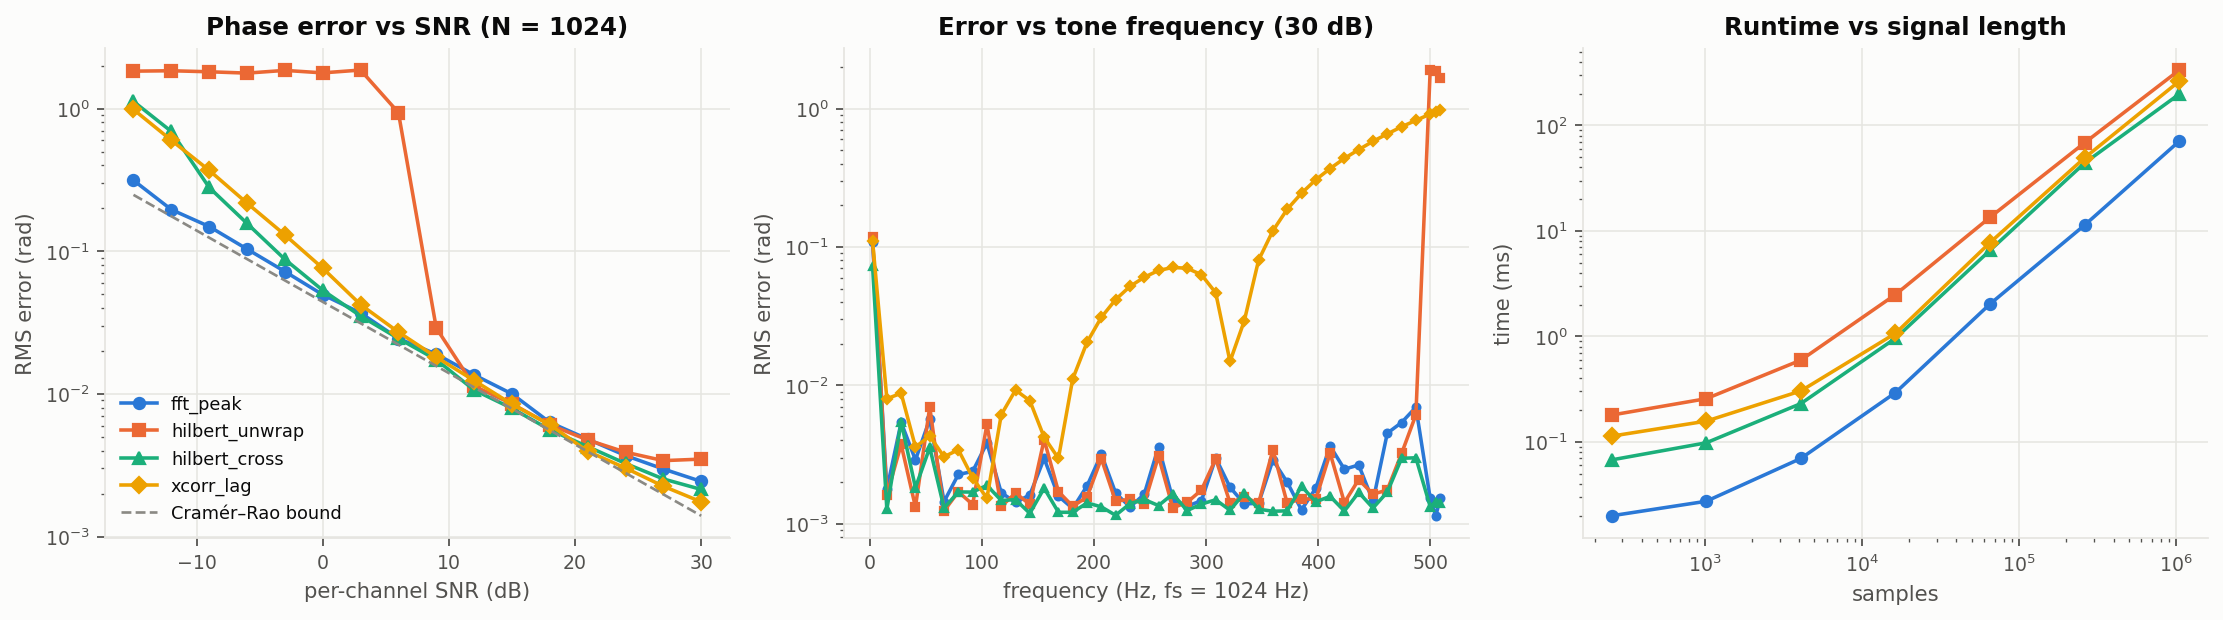
\includegraphics[width=\linewidth]{phase_estimators.png}
  \caption{Two-tone phase estimators. Left: RMS error against SNR, with the Cramér--Rao bound
  (dashed). Middle: error against tone frequency at \SI{30}{dB}. All methods degrade near DC. The
  lag method degrades steadily towards Nyquist because parabolic peak interpolation becomes biased
  with fewer samples per period, and Hilbert unwrapping fails at Nyquist. Right: runtime against
  signal length.}
  \label{fig:phase}
\end{figure}

The original comparison is repeated with Monte-Carlo trials, phase-wrapped errors and an
off-bin tone (\SI{97.3}{Hz} at $f_s=\SI{1024}{Hz}$, $N=1024$). Figure~\ref{fig:phase} compares four
estimators: the cross-spectrum at the FFT peak bin, the legacy Hilbert method (mean of the unwrapped
instantaneous-phase difference), the averaged analytic cross-product $\arg\sum a_2a_1^*$, and the
cross-correlation lag (with the legacy whole-sample quantisation removed). For a tone in white noise,
any unbiased estimator obeys
\begin{equation}
\operatorname{var}(\hat\varphi_2-\hat\varphi_1)\ge\frac{2}{N\cdot\mathrm{SNR}},\qquad
\mathrm{SNR}=\frac{A^2}{2\sigma^2}.
\end{equation}
The cross-product estimators follow the bound down to low SNR. At \SI{0}{dB} the analytic
cross-product reaches \HilbertCrossZeroDb\,rad, against a bound of \CrlbZeroDb\,rad. The legacy
unwrapping method breaks down: a single $2\pi$ slip biases the whole mean, and its error at
\SI{0}{dB} is \HilbertUnwrapZeroDb\,rad.

All four estimators assume a single tone, but a real sky signal is broadband noise. The estimator
that generalises is the cross-product evaluated separately in every frequency channel, which is
exactly the FX correlator.

%----------------------------------------------------------------------------------------------
\section{The FX correlator}\label{sec:corr}

The F-step splits each stream into blocks of $n_{\mathrm{chan}}$ samples and applies a unitary FFT to
each. The X-step then averages $X_iX_j^*$ over blocks for every baseline and channel. For $S$
samples per receiver the X-step performs $\tfrac12N(N-1)S$ complex multiply--accumulates (8 real
flops each) and dominates for $N\gtrsim8$. Every back end exposes the same call,
\texttt{correlate(volts, nchan, backend)}:

\begin{center}\small
\begin{tabular}{ll}
\toprule
back end & X-step implementation\\
\midrule
\texttt{numpy-loop} & one baseline at a time, vectorised over channels\\
\texttt{numpy-gemm} & per channel $R=SS^H$ (batched BLAS \texttt{cgemm})\\
\texttt{torch-cpu/cuda} & the same GEMM formulation in PyTorch\\
\texttt{c-scalar} & plain C, auto-vectorisation disabled (reference)\\
\texttt{c-avx2} & AVX2+FMA intrinsics, 8 channels per iteration\\
\texttt{c-avx2-omp} & as above, OpenMP across baselines\\
\bottomrule
\end{tabular}
\end{center}

The AVX2 kernel avoids a shuffle per complex product. A \texttt{\_\_m256} register holds four
interleaved complex values, and the kernel accumulates $P \mathrel{+}= a\odot b$ and
$Q \mathrel{+}= a\odot\mathrm{swap}(b)$ with fused multiply--adds over all blocks. Only at the end does
it form $\mathrm{Re}=P_{\text{even}}+P_{\text{odd}}$ and $\mathrm{Im}=Q_{\text{odd}}-Q_{\text{even}}$,
the real and imaginary parts of $a\,\bar b$.

The memory layout turned out to matter more than the arithmetic. A first version walked the spectra
baseline by baseline. It re-read each antenna $N-1$ times from DRAM with a stride of
$8\,n_{\text{chan}}$ bytes, reached only about 5\,GFLOP/s, and did not speed up with more threads
because every core competed for the same memory bandwidth. The final kernel is cache-blocked. It
copies an 8-channel block of all antennas into a contiguous buffer (one 64-byte line per antenna and
time step), forms every baseline from it while it sits in L1/L2, and register-tiles two baselines per
load. OpenMP then parallelises over channel blocks. This raised single-core throughput about fourfold
and made the kernel scale with cores. All back ends agree with the reference to float32 precision
(tests in \texttt{tests/test\_correlator.py}).

\begin{figure}[t]
  \centering
  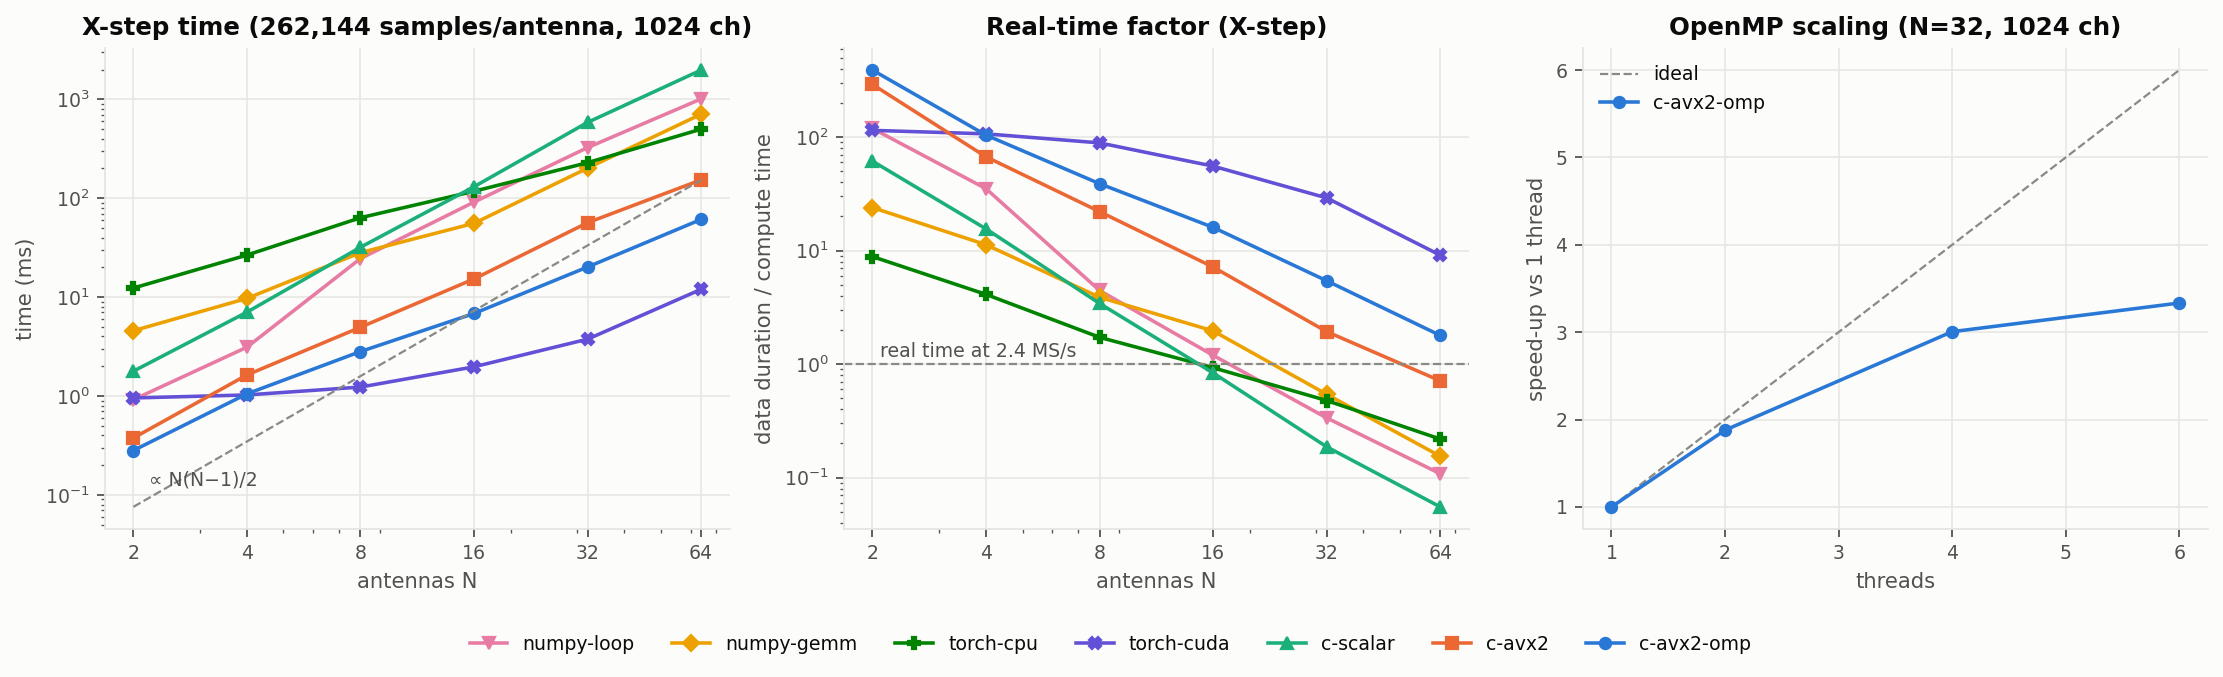
\includegraphics[width=\linewidth]{correlator_scaling.png}
  \caption{X-step time (left) and real-time factor (middle) against the number of receivers, at
  1024 channels and \NSamples\ samples per receiver. Right: OpenMP thread scaling at $N=32$.}
  \label{fig:corr}
\end{figure}

\begin{table}[t]
\centering\small
\caption{X-step real-time factor at 2.4\,MS/s per receiver, 1024 channels (higher is better; $>1$ keeps up with a live stream). \texttt{torch-cuda} measured on a cloud GPU, other rows on the CPU host; --: skipped (estimated $>$20\,s); pending: no GPU results available.}
\label{tab:corr}
\begin{tabular}{lrrrrrr}
\toprule
back end & $N=2$ & $N=4$ & $N=8$ & $N=16$ & $N=32$ & $N=64$ \\
\midrule
\texttt{numpy-loop} & 119 & 35 & 4.45 & 1.2 & 0.336 & 0.108 \\
\texttt{numpy-gemm} & 23.9 & 11.2 & 3.88 & 1.96 & 0.542 & 0.154 \\
\texttt{torch-cpu} & 8.84 & 4.11 & 1.72 & 0.929 & 0.477 & 0.219 \\
\texttt{torch-cuda} & 114 & 106 & 88.7 & 55.3 & 29.1 & 9.1 \\
\texttt{c-scalar} & 61.3 & 15.5 & 3.42 & 0.836 & 0.187 & 0.0553 \\
\texttt{c-avx2} & 290 & 66.8 & 22 & 7.15 & 1.93 & 0.712 \\
\texttt{c-avx2-omp} & 388 & 104 & 38.8 & 16 & 5.41 & 1.79 \\
\bottomrule
\end{tabular}
\end{table}


Figure~\ref{fig:corr} and Table~\ref{tab:corr} summarise the results. The cost follows the expected
$N(N-1)/2$ curve. Explicit SIMD gives a $\SpeedupAvxScalar\times$ gain over scalar C at $N=16$, and
OpenMP adds a further $\ThreadSpeedup\times$ on \ThreadsMax\ threads, peaking at
\GflopsOmpPeak\,GFLOP/s. At $N=64$ (2016 baselines) the AVX2+OpenMP kernel is
$\SpeedupOmpGemmSixtyFour\times$ faster than the NumPy GEMM formulation. That formulation is limited
by the small, skinny matrices involved ($N\times n_{\text{spec}}$ per channel), which suit BLAS poorly
on a CPU but suit GPUs well.

The same GEMM formulation in PyTorch was run on a cloud GPU (\GpuHost, via
\texttt{benchmarks/gpu\_colab.ipynb}). Each call has a floor of about \SI{1}{ms} from kernel
launches and the baseline gather, so for two to four receivers the CPU kernel is as fast or faster.
From $N=8$ the GPU pulls ahead. At $N=64$ it reaches \GflopsCudaPeak\,GFLOP/s and
\RtfCudaSixtyFour$\times$ real time, $\SpeedupCudaOmpSixtyFour\times$ faster than the AVX2+OpenMP
kernel. These timings exclude host--device transfers. In a deployment the spectra would be produced
on the GPU (F-step there too), so only the visibilities would need to come back.

%----------------------------------------------------------------------------------------------
\section{Real-time streaming correlator}\label{sec:stream}

The original C prototype streamed two sine waves over TCP. Its receiving threads wrote into shared
buffers without holding the lock, never matched blocks between receivers, and rebuilt FFTW plans for
every block. The replacement has two programs:

\begin{itemize}
\item \texttt{rx\_sim} simulates $N$ receivers, each a thread with its own TCP connection. Each sends
32-byte headers (antenna id, sequence number, timestamp) followed by 4096 samples of 8-bit I/Q, as an
SDR would. All receivers start their sample clocks at a common epoch, as GPS-locked receivers would.
Senders either run on a fixed schedule or go as fast as TCP back-pressure allows. On a fixed
schedule, a frame that back-pressure delays beyond a 32-frame (\SI{55}{ms}) receiver buffer is
counted as an \emph{overrun}, i.e.\ data a real receiver would lose.
\item \texttt{corrd} runs one receiving thread per connection. Each thread writes complete frames
into a per-receiver ring buffer under a lock and blocks when it is \texttt{ring} frames ahead, so no
data are dropped silently. A correlator thread waits until frame $s$ has arrived from \emph{every}
receiver and unpacks it into the current integration. Every 16 frames it runs the F-step (a
pre-planned radix-2 FFT, parallel over receivers) and \emph{one} AVX2 X-step over the whole
integration, then writes a visibility dump. Integration is simply a longer sum in the X-step.
\end{itemize}

\begin{figure}[t]
  \centering
  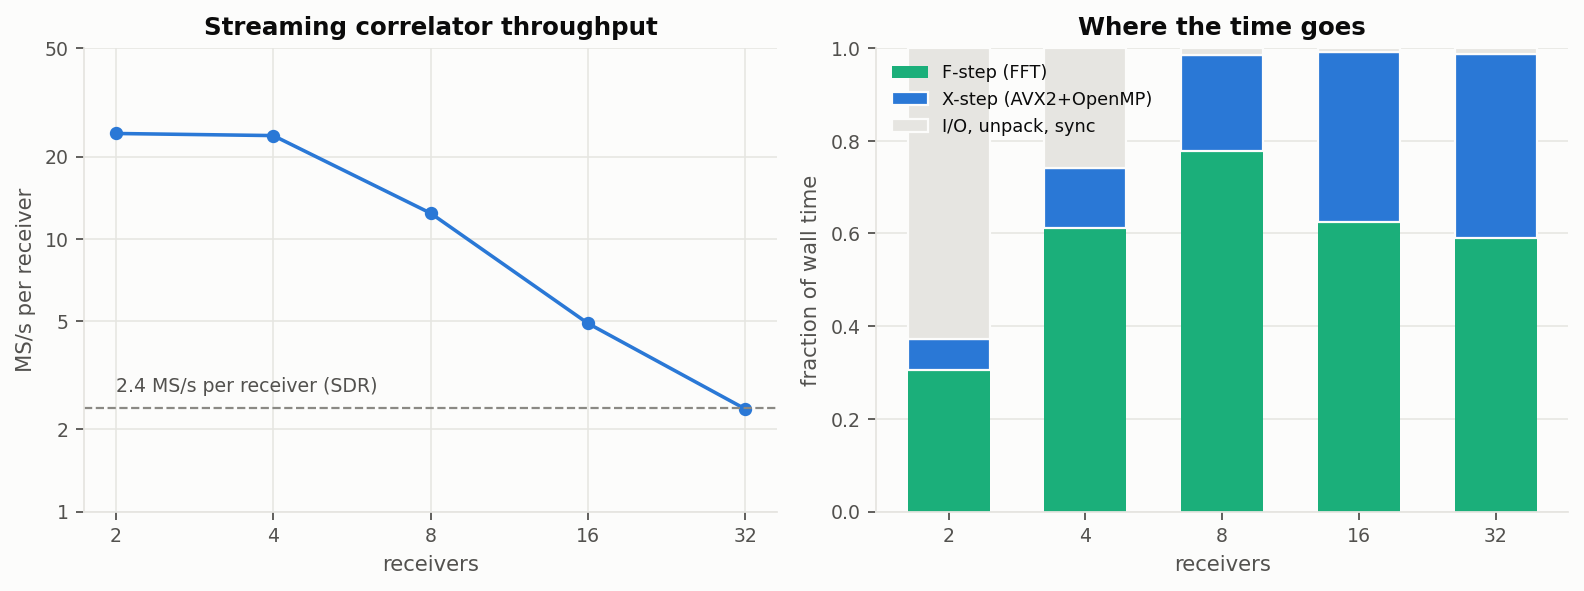
\includegraphics[width=0.9\linewidth]{stream_throughput.png}
  \caption{Streaming daemon on one machine (localhost). Left: sustained throughput per receiver,
  including sockets, unpacking, FFT and X-step. Right: share of wall time per stage.}
  \label{fig:stream}
\end{figure}

Three engineering iterations were needed to make the daemon real-time:
\begin{enumerate}
\item Calling the multi-threaded X-step once per 4096-sample frame spent most of the time in OpenMP
fork/join, so it reached only 2.2\,MS/s per receiver at $N=8$. Batching a whole integration into one
call, with a parallel FFT, fixed that.
\item Each simulated receiver originally started its clock when it connected. Early receivers ran
ahead, were throttled by the alignment window, and showed spurious lag. A common start epoch fixed
that.
\item With the OpenMP pool on all hardware threads, the 32 socket threads (senders and receivers)
were starved during compute bursts. With the pool limited to half the CPUs, 16 receivers went from
hundreds of overruns to none.
\end{enumerate}
On one machine, sharing the CPU with the simulated senders, the daemon sustains \StreamMspsTwo,
\StreamMspsEight, \StreamMspsSixteen\ and \StreamMspsThirtyTwo\,MS/s per receiver for 2, 8, 16 and
32 receivers (Figure~\ref{fig:stream}). That is $5\times$ real time at $N=8$, $2\times$ at $N=16$,
and right at the limit for $N=32$. Paced at \SI{2.4}{MS/s}, the 8- and 16-receiver runs had
\StreamOverrunsEight\ and \StreamOverrunsSixteen\ overruns, with maximum lags of \StreamMaxLagEight\
and \StreamMaxLagSixteen\,ms. In this regime the simple radix-2 FFT, not the correlation, takes
most of the time (right panel), so an optimised FFT library would be the next improvement. The dumps
match the offline NumPy correlator on the same quantised samples to a relative difference of about
$10^{-6}$.

%----------------------------------------------------------------------------------------------
\section{Imaging and calibration}\label{sec:imaging}

\begin{figure}[t]
  \centering
  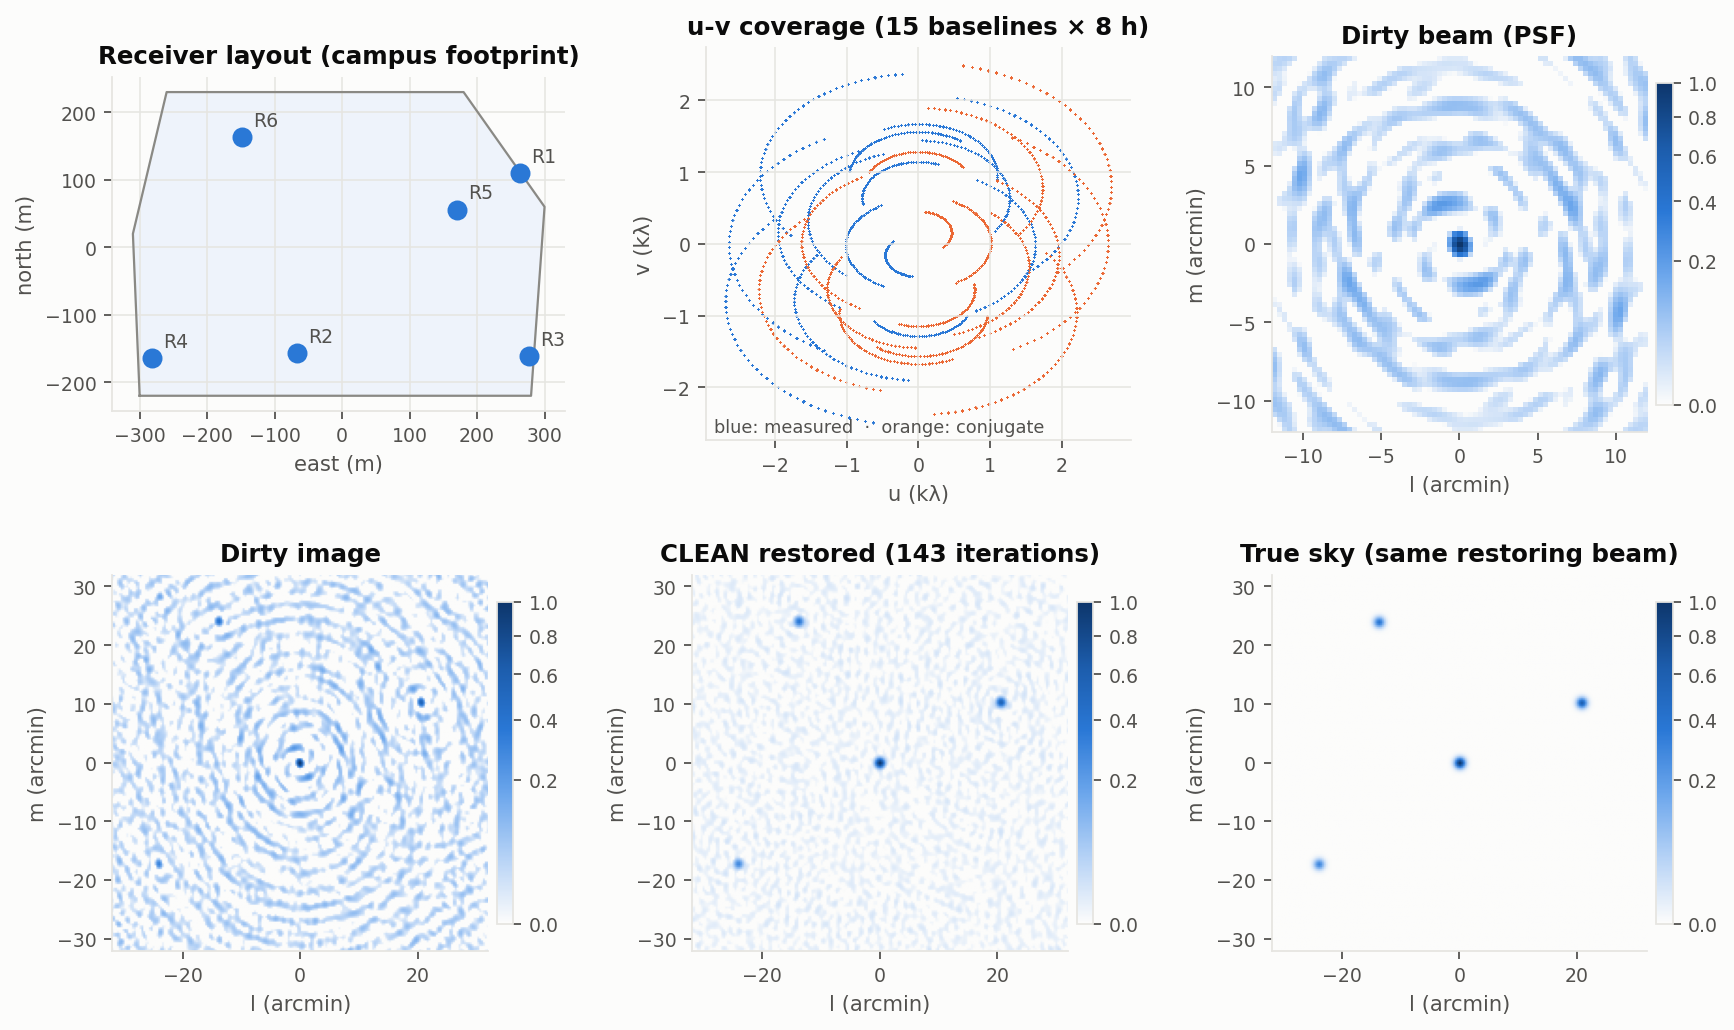
\includegraphics[width=\linewidth]{imaging.png}
  \caption{End-to-end simulation: six receivers on the campus footprint, 48 correlator snapshots
  over 8 hours, gridding, dirty image, and Högbom CLEAN. Images use a square-root stretch.}
  \label{fig:imaging}
\end{figure}

Visibilities from all snapshots and channels are gridded onto a fourfold-oversampled $(u,v)$ grid.
Oversampling suppresses the phase errors of nearest-neighbour gridding away from the phase centre.
The inverse FFT gives the dirty image, the true sky convolved with the dirty beam.
Figure~\ref{fig:imaging} shows the full pipeline starting from simulated voltages: the 15 baselines
trace arcs in the $(u,v)$ plane, and the resulting dirty beam (FWHM about 1.1 arcmin) has sidelobes of
about 0.2. Högbom CLEAN removes them and recovers the four source fluxes (1.0, 0.6, 0.4, 0.3) to within
about 5\,\%. The w-term is neglected, which is accurate for fields within about \ang{0.5} on these
baselines. A wider field would need w-projection.

\begin{figure}[t]
  \centering
  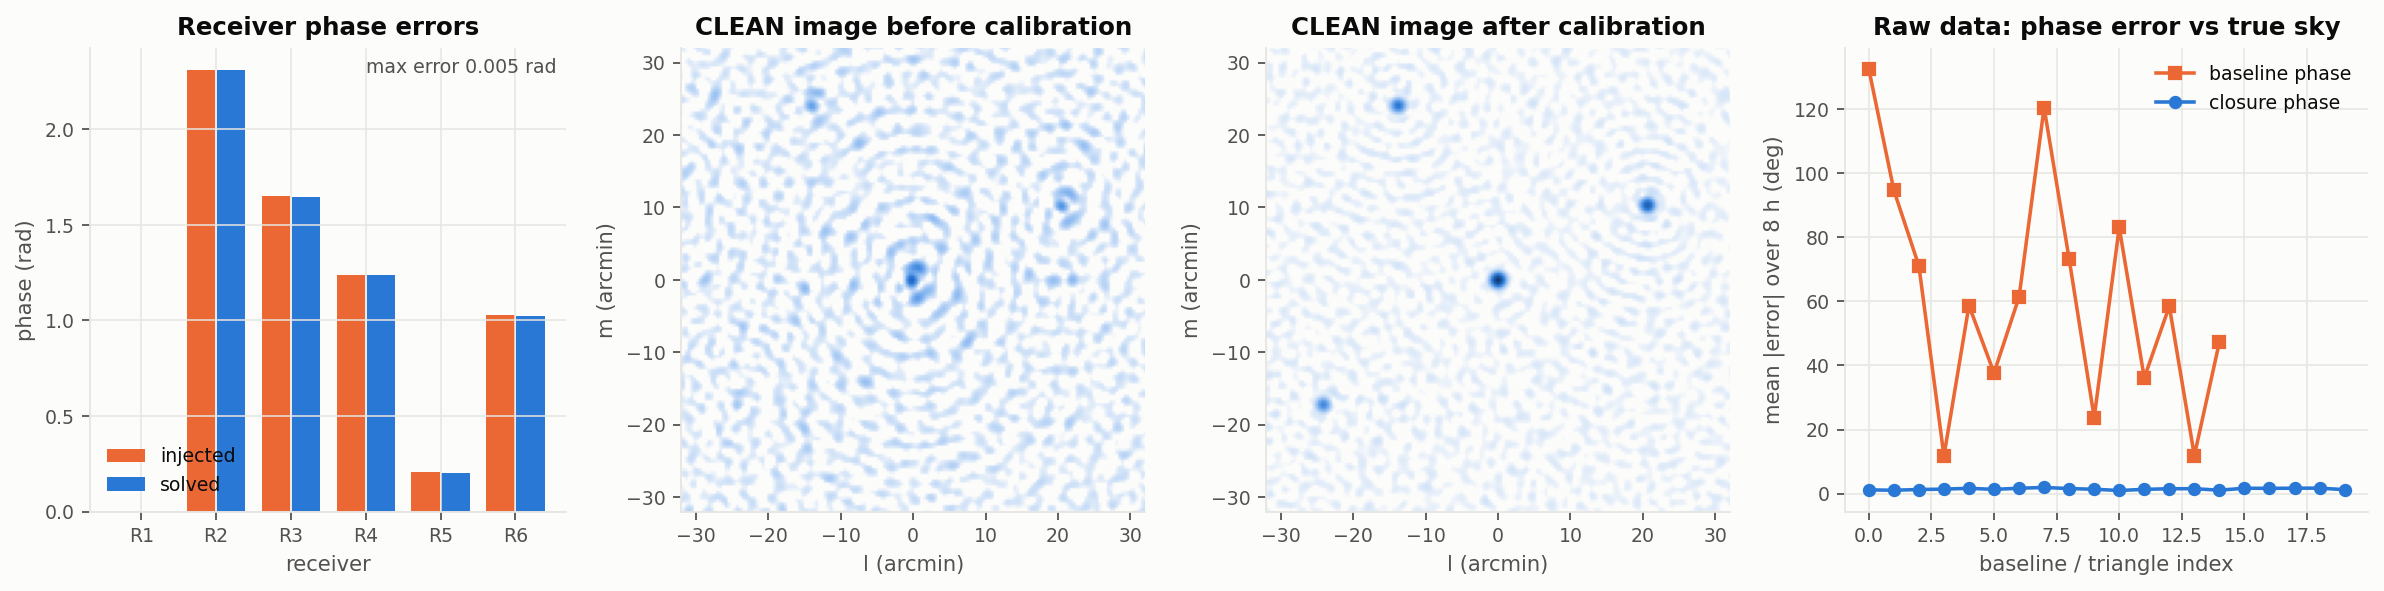
\includegraphics[width=\linewidth]{calibration.png}
  \caption{Gain calibration. Receivers are given $\sim$1\,rad phase and 10\,\% amplitude errors.
  StEFCal solves them from a short calibrator scan, which restores the image. Closure phases of the
  raw data match the true sky, whereas baseline phases do not.}
  \label{fig:cal}
\end{figure}

Real receivers add unknown complex gains (cable lengths, amplifiers, local oscillators), so
$V^{\text{obs}}_{ij}=g_ig_j^*V_{ij}$. With $N$ unknowns and $N(N-1)/2$ measurements, a short
observation of a calibrator at the phase centre fixes the gains. StEFCal, an alternating
least-squares solver, recovers injected phase errors of about 1\,rad to within \SI{0.005}{rad}
(Figure~\ref{fig:cal}). Closure phases summed around baseline triangles cancel all antenna phases
exactly. They stay within noise (about \ang{1.5}) of the true sky, while uncorrected baseline phases
are off by about \ang{60} on average.

%----------------------------------------------------------------------------------------------
\section{Where to put the receivers}\label{sec:layout}

\begin{figure}[t]
  \centering
  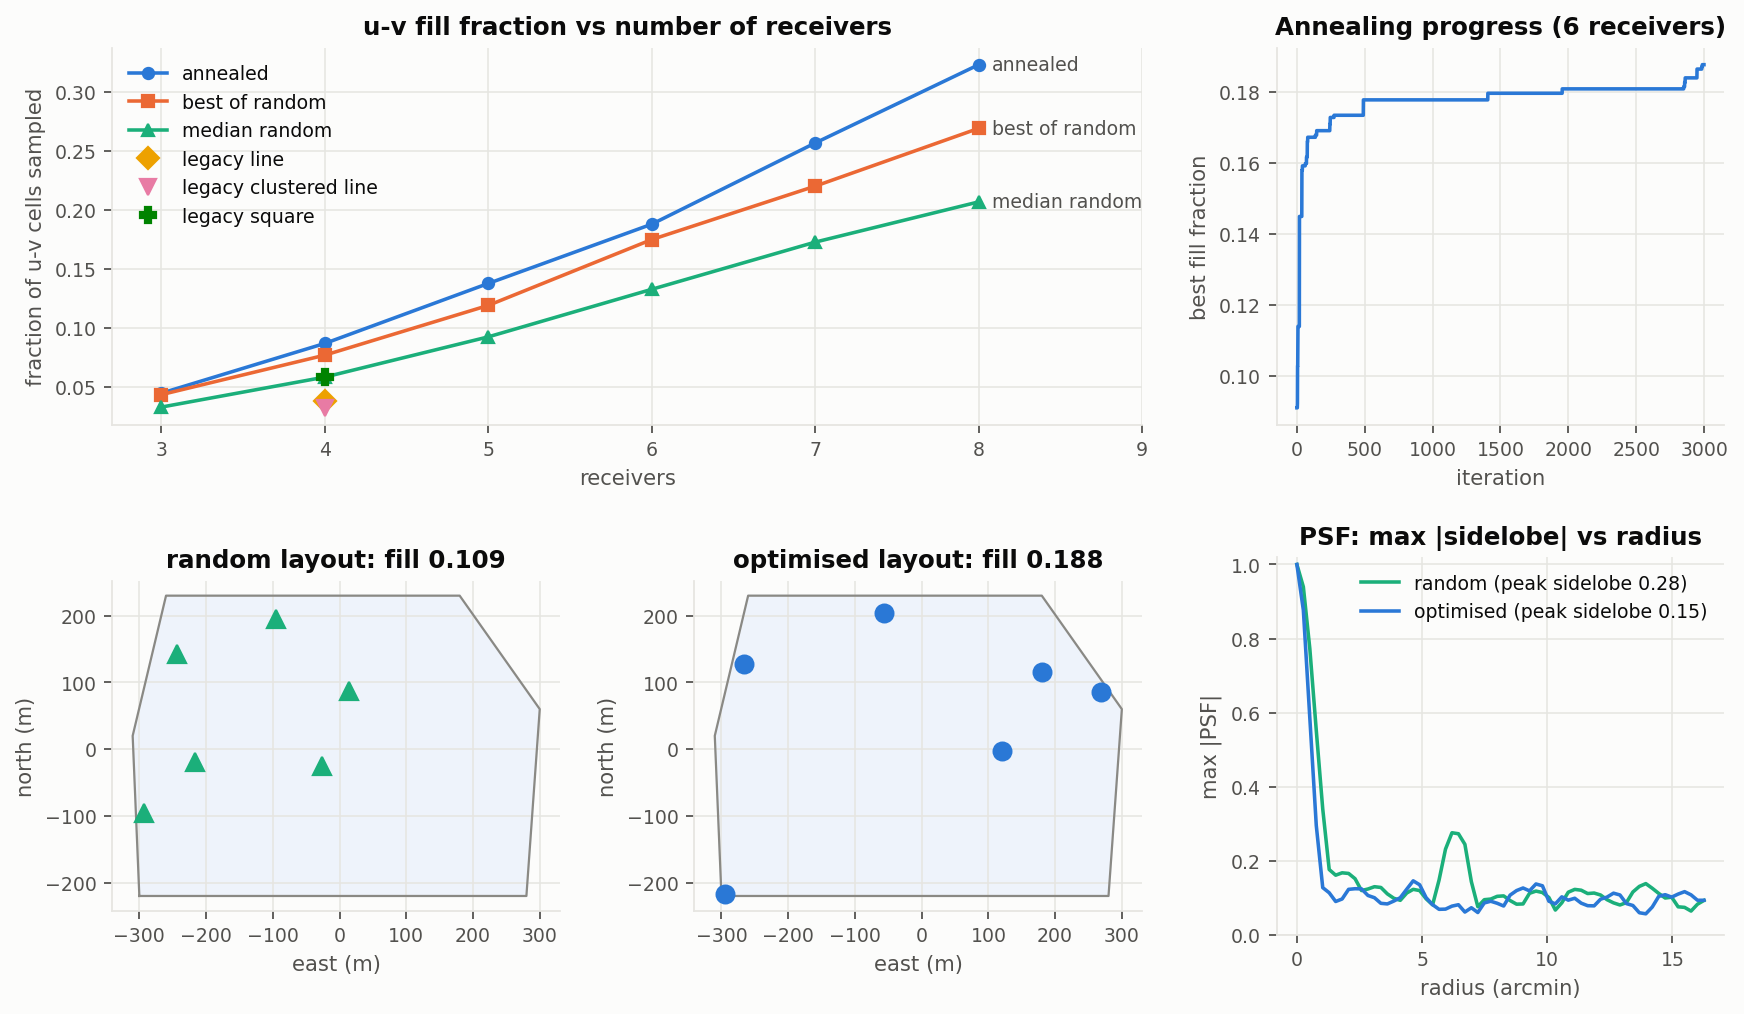
\includegraphics[width=\linewidth]{layout.png}
  \caption{Layout optimisation. Top: $(u,v)$ fill fraction against the number of receivers for the
  original hand-made layouts, random placements and simulated annealing. Bottom: a random and an
  optimised 6-receiver layout and the radial sidelobe envelope of their dirty beams.}
  \label{fig:layout}
\end{figure}

The original notebook scored layouts by plotting their $(u,v)$ tracks and counting dark pixels. Here
the same idea is computed directly. The score is the fraction of cells of a $64\times64$ $(u,v)$ grid,
within the disk the campus can reach, that the Earth-rotation tracks visit. Simulated annealing then
moves one receiver at a time inside the campus polygon, keeping a minimum separation of \SI{15}{m}.
With four receivers, the original square layout fills \LayoutLegacySquare\ and the line
\LayoutLegacyLine, while annealing reaches \LayoutAnnealFour. With eight receivers, annealing reaches
\LayoutAnnealEight, against \LayoutRandBestEight\ for the best of 200 random layouts and
\LayoutRandMedEight\ for the median (Figure~\ref{fig:layout}). Better coverage translates directly
into lower dirty-beam sidelobes, which makes CLEAN's job easier.

%----------------------------------------------------------------------------------------------
\section{Limitations and future work}

\begin{itemize}
\item \textbf{GPU timings} exclude host--device copies and come from a shared cloud GPU; the streaming
daemon itself is CPU-only. Moving the F- and X-steps of \texttt{corrd} to the GPU, ideally with
tensor-core GEMMs, is the natural next step for arrays beyond about 16 receivers.
\item \textbf{Single-machine streaming.} The receivers and the correlator share one CPU over
loopback, and streaming time is dominated by a simple radix-2 FFT; FFTW or a batched SIMD FFT
would raise the receiver count further. A real deployment needs distributed receivers, a common clock (GPS-disciplined oscillators
or White Rabbit), and coarse delay correction before correlation.
\item \textbf{Imaging simplifications.} The imager uses nearest-neighbour gridding, no w-term, no
primary-beam correction, and point sources only.
\item \textbf{No real data.} No real data were recorded. The natural next step is to replay
recordings from the campus receivers through \texttt{rx\_sim --input}.
\item \textbf{Possible extensions.} Polyphase filter banks instead of a plain FFT; RFI flagging;
tensor-core correlation; redundant-baseline calibration; HI-line spectral imaging.
\end{itemize}

%----------------------------------------------------------------------------------------------
\section{Reproducing the results}
\begin{lstlisting}
make lib       # C library + streaming tools (gcc, OpenMP, AVX2)
make test      # pytest suite
make examples  # figures in figs/
make bench     # benchmarks/results/*.csv
make report    # this document
\end{lstlisting}

\begin{thebibliography}{9}\small
\bibitem{tms} A.\,R.~Thompson, J.\,M.~Moran, G.\,W.~Swenson, \emph{Interferometry and Synthesis in
Radio Astronomy}, 3rd ed., Springer (2017).
\bibitem{sira} G.\,B.~Taylor, C.\,L.~Carilli, R.\,A.~Perley (eds.), \emph{Synthesis Imaging in Radio
Astronomy II}, ASP Conf.\ Ser.\ 180 (1999).
\bibitem{hogbom} J.\,A.~Högbom, Aperture synthesis with a non-regular distribution of interferometer
baselines, \emph{A\&AS} 15, 417 (1974).
\bibitem{stefcal} S.~Salvini, S.\,J.~Wijnholds, Fast gain calibration in radio astronomy using
alternating direction implicit methods, \emph{A\&A} 571, A97 (2014).
\bibitem{kay} S.\,M.~Kay, \emph{Fundamentals of Statistical Signal Processing: Estimation Theory},
Prentice Hall (1993).
\bibitem{xgpu} M.\,A.~Clark, P.\,C.~La Plante, L.\,J.~Greenhill, Accelerating radio astronomy
cross-correlation with graphics processing units, \emph{IJHPCA} 27(2), 178 (2013).
\end{thebibliography}

\end{document}
